\documentclass[11pt]{article}

%%%%%%%%%%%%%%%%%%%
% Page Layout
%%%%%%%%%%%%%%%%%%%

\setlength{\paperwidth}{8.5in} \setlength{\paperheight}{11in}
\setlength{\marginparwidth}{0in} \setlength{\marginparsep}{0in}
\setlength{\oddsidemargin}{0in} \setlength{\evensidemargin}{0in}
\setlength{\textwidth}{6.5in} \setlength{\topmargin}{-0.5in}
\setlength{\textheight}{9in}

%%%%%%%%%%%%%%%%%%%%%%%%%%%%%%%%%%%
% Include Packages and Style Files
%%%%%%%%%%%%%%%%%%%%%%%%%%%%%%%%%%%

\usepackage[english]{babel}
\usepackage{amsmath,amssymb,amsthm}
\usepackage{enumerate}
\usepackage[useregional]{datetime2}
\usepackage[pdftex]{graphicx,color}
\usepackage{multicol}
\setlength{\columnsep}{1.5cm}
\usepackage{algorithm2e}
\usepackage{listings}
\usepackage{multirow}
\usepackage[utf8]{inputenc}
\usepackage[bottom]{footmisc}
\usepackage{animate}
\usepackage{float}
\usepackage{hyperref}

\hypersetup{
    colorlinks=true,
    linkcolor=blue,
    filecolor=magenta,
    urlcolor=cyan,
}
\urlstyle{same}

\setlength{\arrayrulewidth}{0.8mm}
\setlength{\tabcolsep}{18pt}
\renewcommand{\arraystretch}{1.25}

%%%%%%%%%%%%%%%%%%%%%%%%%%%%%%
% Define theorem environments
%%%%%%%%%%%%%%%%%%%%%%%%%%%%%%

\newtheorem{theorem}{Theorem}[section]
\newtheorem{proposition}[theorem]{Proposition}
\newtheorem{lemma}[theorem]{Lemma}
\newtheorem{corollary}[theorem]{Corollary}
\newtheorem{claim}[theorem]{Claim}
\newtheorem{question}[theorem]{Question}
\newtheorem{conjecture}[theorem]{Conjecture}

\theoremstyle{definition}
\newtheorem{definition}[theorem]{Definition}
\newtheorem{example}[theorem]{Example}
\newtheorem*{remark}{Remark}

%%%%%%%%%%%%%%%%%%%%%%
% Define new commands
%%%%%%%%%%%%%%%%%%%%%%

\newcommand{\R}{\mathbb{R}}


\newcommand{\E}{\mathbb{E}}
\renewcommand{\P}{\mathbb{P}}
\newcommand{\Var}{\operatorname{Var}}
\newcommand{\1}[1]{\mathbf{1} \left \{ #1 \right \}}
\newcommand{\Range}{\operatorname{Range}}

%%%%%%%%%%%%%%%%%%%%%%

\begin{document}

\title{Numerical Analysis Project \\ MATH 5600 \\ Homework 2}
\date{Due: March 3, 2021}
\author{Authors: \\ Dane Gollero $\cdot$ Ike Griss Salas $\cdot$ Magon Bowling}

\maketitle

\tableofcontents

\section{Homework Problems}

\begin{itemize}
    \item[{\textbf{-1-}}] \textbf{(Taylor Series.)}  Let
    \begin{equation}
        f(x)=e^x \text{ and } g(x)=\ln(x+1)
    \end{equation}
    and let $p_n$ and $q_n$ be the Taylor polynomials of degree $n$ for $f$ and $g$, respectively, about
    \begin{equation}
        x_0 = 0.
    \end{equation}
    Plot the graphs of $f$, $g$, $p_n$ and $q_n$, for some small values of $n$, and comment on your results.  Discuss in particular how well $f$ and $g$ are approximated by their Taylor polynomials.  Explain your observations in terms of a suitable expression for the error in the approximation.
\end{itemize}
Recall the Taylor Series
\[f(x) = \sum_{i=0}^{\infty} f^{(i)} (\alpha) \cdot \frac{(x-\alpha)^i}{i!}.\]
We know that for all \(i \in \mathbb{N}\),
\[f(x) = e^x \Rightarrow f^{(i)}(0) = 1.\]
Thus,
\[f(x) = e^x = \sum_{i=0}^{\infty} \frac{x^i}{i!}.\]
We also have
\begin{equation*}
    \begin{split}
        g(x) &= \ln (x+1) = 0 \quad \text{for } x = 0 \\
        g^{\prime}(x) &= \frac{1}{x+1} = 1 = 1! \qquad \text{at} \ x = 0 \\
        g^{\prime\prime}(x) &= \frac{-1}{(x+1)^2} = -1 = -1! \qquad \text{at} \ x = 0 \\
        g^{\prime\prime\prime}(x) &= \frac{2}{(x+1)^3} = 2 = 2! \qquad \text{at} \ x = 0 \\
        g^{(4)}(x) &= \frac{-6}{(x+1)^4} = -6 = -3! \qquad \text{at} \ x = 0 \\
        \vdots \\
        g^{(n)} (x) &= \frac{(-1)^{n-1} (n-1)!}{(x+1)^n} = (-1)^{n-1} (n-1)! \quad \text{for } x=0, n>0
    \end{split}
\end{equation*}
\[\Longrightarrow \sum_{n=1}^{\infty} (-1)^{n-1} (n-1)! \cdot \frac{x^n}{n!}.\]
Below, we will illustrate some Taylor polynomial approximations for $f$ and $g$, respectively.\footnote{Code in Appendix -A-.}
\begin{figure}[H]
    \centering
    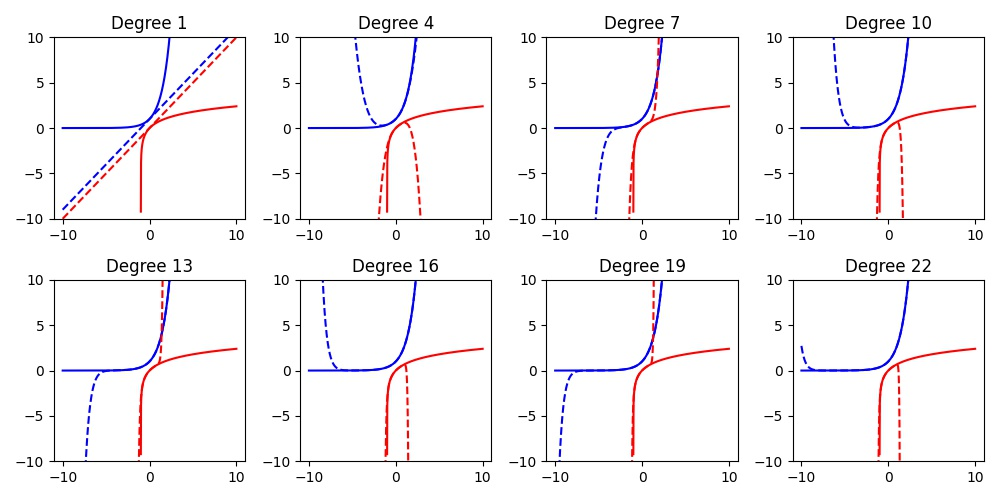
\includegraphics[width=15cm]{hw2_images/8subplots.jpg}
    \caption{Solid Blue indicates $e^x$, Solid Red indicates $\ln(x+1)$, and the Dashed lines represent their Taylor approximations respectively.}
    \label{fig:my_label}
\end{figure}
We show a GIF of the Taylor polynomial approximations here:
\href{https://github.com/3rundane/Numerical-Analysis-Project/blob/main/homework\%202\%20gifs/problemgif.gif}{Taylor Polynomial GIF} \\

Qualitatively we can see the Taylor polynomial, $p_n$, begins to better approximate $e^x$ as $n$ gets larger.  However, the Taylor polynomial, $q_n$, tends to be problematic for larger $n$.  It seems that $q_n$ doesn't approximate $g(x)$ very well for $x>1$, despite increasing values of $n$.  We define the suitable error functions below.
\[E_n^f (x) = \left|e^x - \sum_{k=0}^n \frac{x^k}{k!}\right|\]
\begin{equation*}
    \begin{split}
        E_n^g (x) &= \left|\ln (x+1) - \sum_{k=1}^n (-1)^{k-1} (k-1)! \cdot \frac{x^k}{k!}\right| \\
        &= \left|\ln (x+1) - \sum_{k=1}^n (-1)^{k-1} \frac{x^k}{k}\right|
    \end{split}
\end{equation*}
We show the graphs for our suitable errors as a function $n$ for fixed $x \geq 1$.\footnote{Code in Appendix -B-.}
\begin{figure}[H]
    \centering
    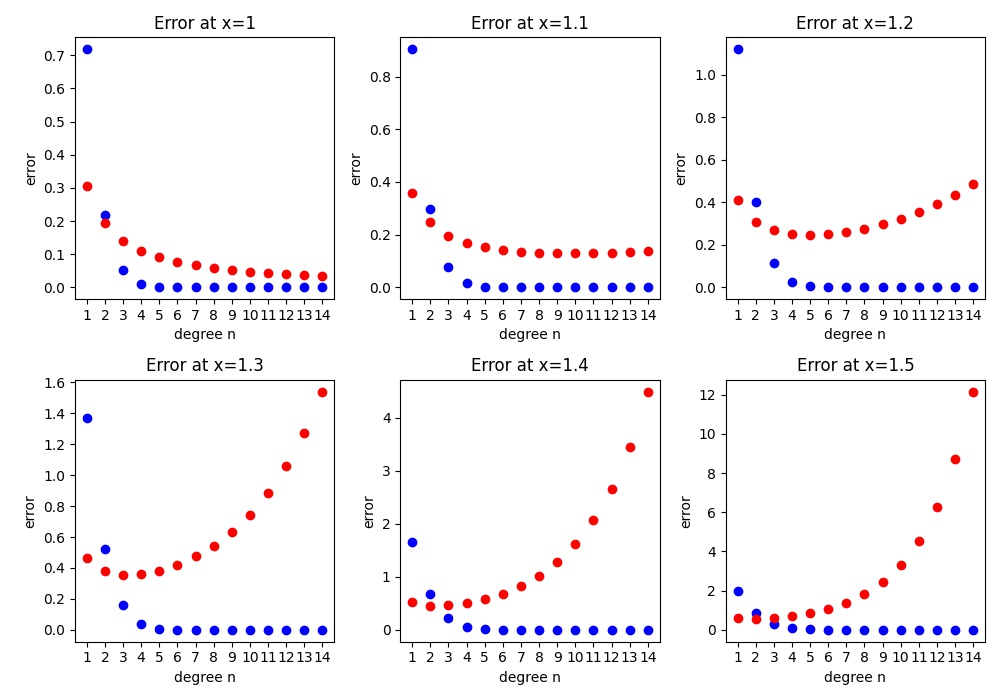
\includegraphics[width=14cm]{hw2_images/error_subplot.jpg}
    \caption{Blue dots indicate the error $E_n^f$ and the Red dots indicate the error $E_n^g$.}
    \label{fig:my_label}
\end{figure}
As we can see increasing our polynomial degree for $q_n$ does not imply a better approximation everywhere.

\begin{itemize}
    \item[{\textbf{-2-}}] \textbf{(A ``simple" program.)}  Write a program that reads $n$ and the entries $x_1$, $x_2$, ..., $x_n$ of a vector $x \in \R^2$ from standard input and prints
    \begin{equation*}
        ||x||_2 = \sqrt{\sum_{i=1}^n x_i^2}
    \end{equation*}
    to standard output.  Mail me your code before the lecture on March 3.
\end{itemize}
\begin{lstlisting}[language=Python]
    from math import sqrt

    def norm(vec):
        square = [i**2 for i in vec]
        square_sum = sum(square)
        size = sqrt(square_sum)
        return size
\end{lstlisting}

\begin{itemize}
    \item[{\textbf{-3-}}] \textbf{(Some Iteration.)}  Consider the iteration
    \begin{equation}
        x_{n+1} = F(x_n) = \sin x_n, \quad x_0 = 1
    \end{equation}
    (where of course the angle is measured in radians).  What does our theory tell us about convergence? Show that the iteration does converge!  What is the limit?  How fast does the iteration converge?  Carefully explain the effects of rounding errors.
\end{itemize}
We have the fixed point iteration $x_{n+1} = g(x_n)$ converges if we have \(\left|g^{\prime} (\alpha)\right| < 1\) where $g(\alpha) = \alpha$, and $x_0$ is sufficiently close to $\alpha$.  In our case, we have $g^{\prime} (\alpha) = \cos (0) = 1$.  On its own this tells us nothing, thus our convergence theory is not particularly helpful.  However, we can say that it indeed converges.  For $x$ on the interval $[0, \frac{\pi}{2}]$ we know that
\[\sin x \leq x.\]
Thus if we assume $x_0$ is sufficiently close to $0$ (on the interval) we have that
\begin{equation*}
    \begin{split}
        x_1 = \sin (x_0) &\leq x_0 \\
        x_2 = \sin (x_1) &\leq \sin (x_0) = x_1 \\
        \vdots
    \end{split}
\end{equation*}
Inductively, we can see $\sin(x)$ is monotonically decreasing on $[0, \frac{\pi}{2}]$.  And we know $\sin(x)$ defined on $[0, \frac{\pi}{2}]$ is bounded below by $0$.  By the Monotone Convergence Theorem, the sequence defined by $x_{n+1} = \sin(x_n)$ converges for $x_0$ sufficiently close to zero.  Furthermore, since $\sin(x)$ is a continuous function on $[0, \frac{\pi}{2}]$ we can say
\[\lim_{x \rightarrow 0^+} \sin (x) = \sin (0) = 0\]
is equivalent to
\[\lim_{n \rightarrow \infty} \sin (x_n).\]
Therefore, our sequence converges to $0$.  This converges much slower than linearly since $g^{\prime} (\alpha) = 1$.  Below we show a table of runtimes for achieving certain error tolerances for this iteration.  \footnote{Runtime will differ for different computers.  Code included in Appendix -C-.}
\begin{center}
\begin{tabular}{ |c|c|c| }
\hline
Error & Steps & Runtime (seconds) \\
\hline
$0.1$ & $295$ & $5.39 \times 10^{-5}$ \\
$0.01$ & $29992$ & $0.005967$ \\
$0.001$ & $2999989$ & $0.677399$ \\
$0.0001$ & $299999986$ & $67.413355$ \\
$0.00001$ & $29999999984$ & $6726.195585$ \\
\hline
\end{tabular}
\end{center}
We can see that $x_{n+1} = \sin (x_n)$ will take a substantial amount of time to converge.  The issues of rounding errors can have catastrophic effects on the ability for our sequence to converge.  If we have a machine that only computes to say the first $3$ decimal points (i.e., it rounds), then the sequence will never converge.  As the iteration progresses, the difference in outputs is less than $3$ decimal places after a certain point, thus, the change in output becomes so minute that the algorithm will not converge to the right value.  In fact, this becomes a constant when running it in Python.  Letting $x_0 = 1$ we have
\begin{center}
\begin{tabular}{ |c|c| }
\hline
 & \(\sin(x_n) = x_{n+1}\) \\
n  & (rounded) \\
\hline
$0$ & $0.841$ \\
$1$ & $0.745$ \\
$2$ & $0.678$ \\
\vdots & \vdots \\
$125$ & $0.145$ \\
$126$ & $0.144$ \\
$127$ & $0.144$ \\
$128$ & $0.144$ \\
\vdots & \vdots \\
\hline
\end{tabular}
\end{center}
The iteration settles on $0.144$ after $126$ steps.  Now of course, we know that $\sin (x_n) = x_{n+1}$ for $x_0 = 1$ does in fact converges to zero from our deeper analysis.  If we simply went to iteration via the computer, we may get misleading results.

\begin{itemize}
    \item[{\textbf{-4-}}] \textbf{Newton's Method}  Suppose $f$ has a root of multiplicity $p>1$ at $x=\alpha$, i.e.,
    \begin{equation}
        f(\alpha) = f^{\prime} (\alpha) = ... = f^{(p-1)} (\alpha) = 0, \quad f^{(p)} (\alpha) \neq 0.
    \end{equation}
    \begin{enumerate}[a.]
        \item Show that Newton's method applied to $f(x) = 0$ converges linearly to $\alpha$.
        \item Show that this modification of Newton's Method:
        \begin{equation}
            x_{k+1} = x_k - p \frac{f(x_k)}{f^{\prime}(x_k)}
        \end{equation}
        converges quadratically to $\alpha$.  \textbf{Hint:}  You probably are thinking of using the Rule of L'Hopital, but the problem is much easier if you think of $f$ as being defined by $f(x) = (x-\alpha)^p F(x)$ where $F(\alpha) \neq 0.$
        \end{enumerate}
\end{itemize}
(a)
\begin{equation*}
    \begin{split}
        g = x - \frac{f}{f^{\prime}} &= x - \frac{(x-\alpha)^p F(x)}{p(x-\alpha)^{p-1} F(x) + (x-\alpha)^p F^{\prime} (x)} \\
        &= x - \frac{(x-\alpha) F(x)}{pF(x) + (x-\alpha)F^{\prime}(x)}
    \end{split}
\end{equation*}
\[g^{\prime} = 1 - \frac{\big(pF(x) + (x-\alpha)F^{\prime}(x)\big) \big(F(x) + (x-\alpha)F^{\prime}(x)\big) - (x-\alpha)F(x) \Big(\big(pF(x) + (x-\alpha)F^{\prime}(x)\big)^2\Big)^{\prime}}{\left(pF(x) + (x-\alpha)F^{\prime}(x)\right)^2}\]
\[g^{\prime}(\alpha) = 1 - \frac{p \cdot F(\alpha) \cdot F(\alpha)}{p^2 \cdot F(\alpha)^2} = 1 - \frac{1}{p} = \left|\frac{p-1}{p}\right| < 1, \quad \text{for all} \ p > 1\]
We have the absolute value of $g^{\prime}(\alpha)$ such that $0 < g^{\prime}(\alpha) < 1$ for all $p>1$.  Thus $f$ converges linearly. \\
(b)
\begin{equation*}
    \begin{split}
        g(x) &= x - p \frac{f}{f^{\prime}} \\
        g^{\prime}(x) &= 1 - p \left(\frac{f}{f^{\prime}}\right)^{\prime} \Longrightarrow g^{\prime}(\alpha) = 1 - p \cdot \frac{1}{p} = 0
    \end{split}
\end{equation*}
This converges at least quadratically.

\begin{itemize}
    \item[{\textbf{-5-}}] \textbf{(Division without division.)}  Suppose you have a computer or calculator that has no built-in division.  Come up with a fixed point iteration that converges to $1/r$ for any given non-zero number $r$, and that only uses addition, subtraction, and multiplication.  \textbf{Hint:}  Write down an equation satisfied by $1/r$, apply Newton's method to that equation, and then modify Newton's method so that it doesn't use division.  Your resulting method should converge of order 2.
\end{itemize}
Let \(f(x) = \frac{1}{x} - r\).  Now $f$ is satisfied by $x = \frac{1}{r}$ for $r \neq 0$.  We have
\begin{equation*}
    \begin{split}
        f(x) &= \frac{1}{x} - r \\
        f^{\prime}(x) &= \frac{-1}{x^2} \\
        f^{\prime\prime}(x) &= \frac{2}{x^3}
    \end{split}
\end{equation*}
Both $f^{\prime}$ and $f^{\prime\prime}$ are non-zero at $x = \frac{1}{r}$ meaning the Newton's method converges quadratically.  We now look at Newton's method:
\begin{equation*}
    \begin{split}
        g(x) &= x - \frac{f}{f^{\prime}} = x - \frac{\frac{1}{x} - r}{\frac{-1}{x^2}} \\
        &= x - (-x + rx^2) \\
        &= 2x - rx^2.
    \end{split}
\end{equation*}
Again, $g(x)$ converges quadratically since $g^{\prime}(x) = 2 - 2rx$ is zero at $x = \frac{1}{r}$, and $g^{\prime\prime}(x) = -2r$ is non-zero for all $x$.  Thus we have a fixed point iteration that does not use division.  Below we show a hypothetical convergence for some $r$.
\[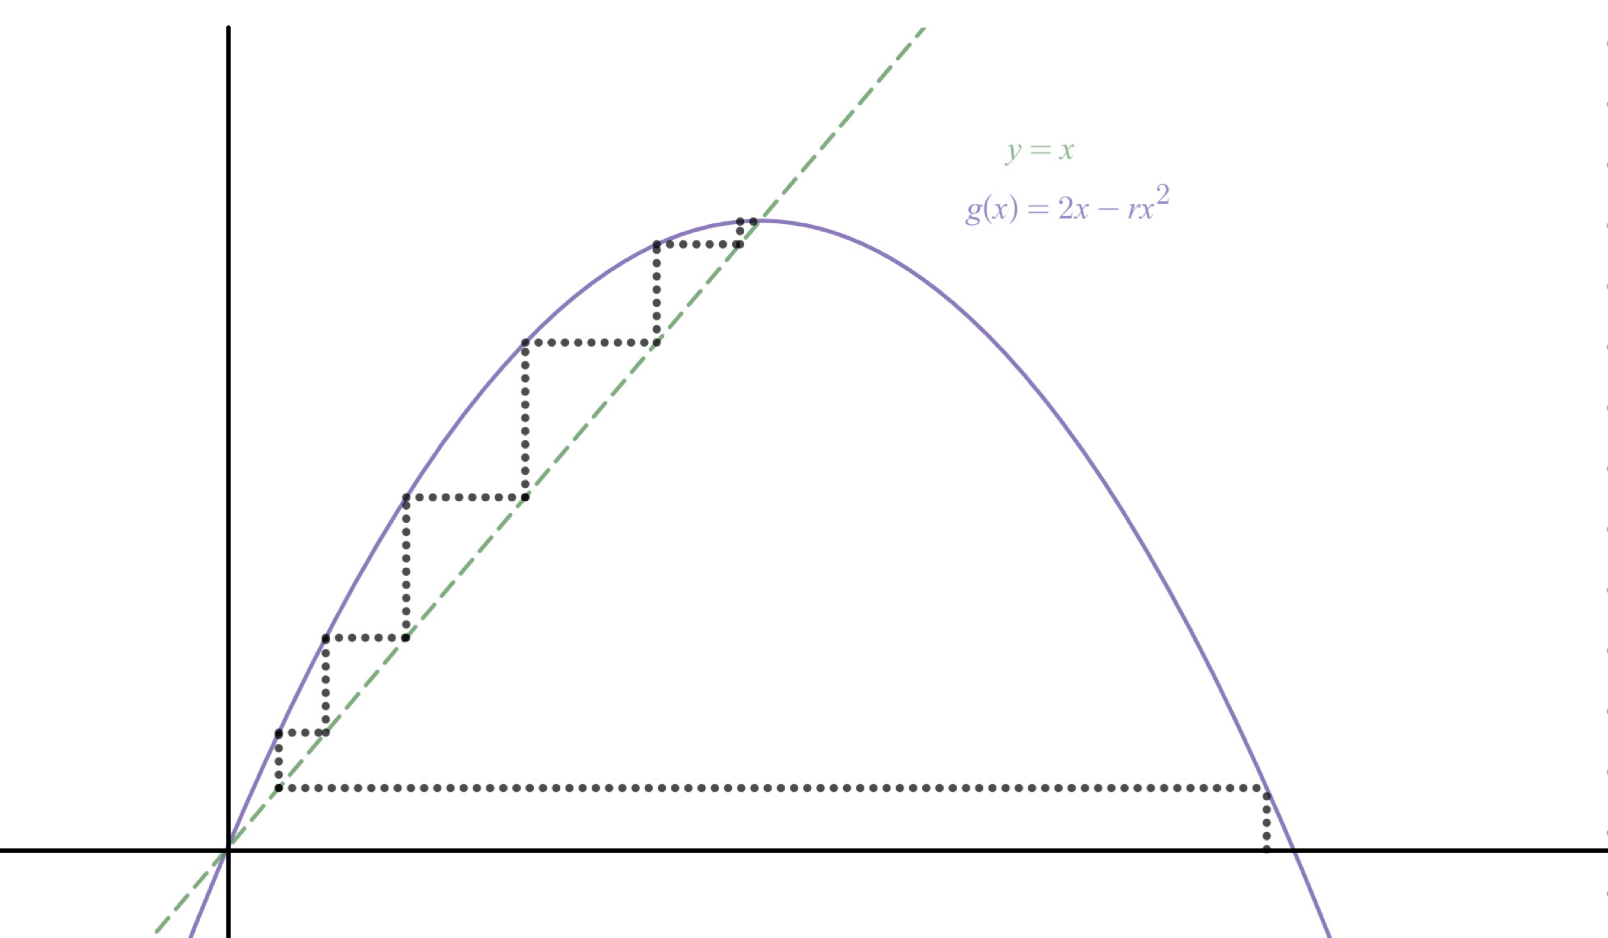
\includegraphics[width=14cm]{hw2_images/convergence.jpg}\]

\begin{itemize}
    \item[{\textbf{-6-}}] \textbf{(A cubically convergent method.)}  Consider the iteration
    \begin{equation*}
        x_{k+1} = g(x_k) \text{  where  } g(x) = x - \frac{f(x)}{f^{\prime}(x)} - \frac{1}{2}\frac{f^2 (x) f^{\prime\prime}(x)}{\left(f^{\prime}(x)\right)^3}.
    \end{equation*}
    (We assume $f$ is sufficiently differentiable, and $f^{\prime}(x) \neq 0$.)  Suppose that $g(\alpha) = \alpha$.  Show that
    \[g^{\prime}(\alpha) = g^{\prime\prime}(\alpha) = 0.\]
    (Thus the fixed point method will converge of order at least $3$ if we start sufficiently close to $\alpha$.)
\end{itemize}
\begin{equation*}
    \begin{split}
        g &= x - \frac{f}{f^{\prime}} - \frac{1}{2} \frac{f^2 f^{\prime\prime}}{f^{\prime 3}} \\
        g^{\prime} &= 1 - \frac{f^{\prime 2} - f f^{\prime\prime}}{f^{\prime 2}} - \frac{1}{2} \frac{f^{\prime 3} (2 f f^{\prime} f^{\prime\prime} + f^2 f^{\prime\prime\prime}) - 3 f^{\prime 2} f^{\prime\prime} f^2 f^{\prime\prime}}{f^{\prime 6}} \\
        &= \frac{f f^{\prime\prime}}{f^{\prime2}} - \frac{1}{2} \frac{2ff^{\prime4}f^{\prime\prime}}{f^{\prime 6}} - \frac{1}{2} \frac{f^2 f^{\prime3} f^{\prime\prime\prime}}{f^{\prime 6}} + \frac{1}{2} \frac{3f^2 f^{\prime2} f^{\prime\prime2}}{f^{\prime 6}} \\
        &= \frac{f f^{\prime\prime}}{f^{\prime2}} - \frac{f f^{\prime\prime}}{f^{\prime 2}} - \frac{1}{2} \frac{f^2 f^{\prime\prime\prime}}{f^{\prime 3}} + \frac{1}{2} \frac{3 f^2 f^{\prime\prime2}}{f^{\prime 4}} \\
        &= \frac{1}{2} f^2 \left(\frac{f^{\prime\prime2}}{f^{\prime4}} - \frac{f^{\prime\prime\prime}}{f^{\prime3}}\right) = 0 \quad \text{at} \ x = \alpha \ \text{since} \ f(\alpha) = 0 \ \text{and} \ f^{\prime}(\alpha) \neq 0 \\
        g^{\prime\prime} &= f f^{\prime} \left(\frac{f^{\prime\prime2}}{f^{\prime4}} - \frac{f^{\prime\prime\prime}}{f^{\prime3}}\right) + \frac{1}{2}f^2 \left(\frac{f^{\prime\prime2}}{f^{\prime4}} - \frac{f^{\prime\prime\prime}}{f^{\prime3}}\right)^{\prime} \\
        &= 0 \quad \text{at $x=\alpha$ since each term has a multiple of $f$ which is $0$ at } \alpha.
    \end{split}
\end{equation*}
Thus our fixed point iteration converges of order at least $3$.

\begin{itemize}
    \item[{\textbf{-7-}}] \textbf{(Polynomial Interpolation.)}  Suppose you want to interpolate to the data $(x_i, y_i), i=0,..., n$ by a polynomial of degree $n$.  Recall that the interpolating polynomial $p$ can be written in its Lagrange form as
    \begin{equation}
        p(x) = \sum_{i=0}^n y_i L_i (x) \text{  where  } L_i (x) = \frac{\prod_{i \neq j}(x - x_j)}{\prod_{i \neq j}(x_i - x_j)}.
    \end{equation}
    Show that
    \begin{equation}
        \sum_{i=0}^n x_i^j L_i (x) = x^j \text{  for  } j=0,..., n.
    \end{equation}
\end{itemize}
We first note that we have $n+1$ data points, thus any polynomial interpolation up to degree $n$ will be unique, assuming each $x_i$ is distinct.  We have the points \(\left(x_i , x_i^j\right) \text{ for } i=0,1,2,...,n\) and where $j$ is a fixed power that can take on the values $j = 0,1,2,...,n$, which lets us interpolate uniquely.  Also, we assume all the points are distinct.  By the construction of these points, the polynomial $x^j$ interpolates our data.  Since the interpolant is unique, we have
\[P(x) = \sum_{i=0}^n x_i^j L_i (x) = x^j \quad \text{for} \ j = 0,1,...,n.\]

\begin{itemize}
    \item[{\textbf{-8-}}] \textbf{(Uniqueness of the interpolating polynomial.)}  Assume you are given the data
    \begin{equation}
        \begin{split}
            x_i &:\quad 1\quad 2\quad 4\quad 8 \\
            y_i &:\quad 1\quad 2\quad 3\quad 4
        \end{split}
    \end{equation}
    Construct the interpolating polynomial using
    \begin{enumerate}[a.]
        \item the power form obtained by solving the Vandermonde system,
        \item the Lagrange form,
        \item the Newton form,\\
        and show that they all yield the same polynomial.
    \end{enumerate}
\end{itemize}
(a) Vandermonde System: We have $4$ nodes, thus we interpolate with polynomial of degree 3:
\[a + bx + cx^2 + dx^3 = y\]
\begin{equation*}
    \begin{split}
    a + b + c + d &= 1 \\
    a + 2b + 4c + 8d &= 2 \\
    a + 4b + 16c + 64d &= 3 \\
    a + 8b + 64c + 512d &= 4
    \end{split}
    \Longleftrightarrow \begin{bmatrix}
    1 & 1 & 1 & 1 \\
    1 & 2 & 4 & 8 \\
    1 & 4 & 16 & 64 \\
    1 & 8 & 64 & 512
    \end{bmatrix} \begin{bmatrix}
    a \\ b \\ c \\ d
    \end{bmatrix} = \begin{bmatrix}
    1 \\ 2 \\ 3 \\ 4 \end{bmatrix}
\end{equation*}
Solving the corresponding augmented matrix reveals
\[\begin{bmatrix} a & b & c & d \end{bmatrix}^T = \begin{bmatrix} -\frac{10}{21} & \frac{7}{4} & -\frac{7}{24} & \frac{1}{56} \end{bmatrix}^T\]
\[\Longrightarrow P(x) = -\frac{10}{21} + \frac{7}{4}x - \frac{7}{24}x^2 + \frac{1}{56}x^3\]
(b) Lagrange Form:
\begin{equation*}
    \begin{split}
        L_0 (x) &= \frac{(x-2)(x-4)(x-8)}{(-1)(-3)(-7)} = \frac{x^3 - 14x^2 + 56x - 64}{-21} \\
        L_1 (x) &= \frac{(x-1)(x-4)(x-8)}{(1)(-2)(-6)} = \frac{x^3 - 13x^2 + 44x - 32}{12} \\
        L_2 (x) &= \frac{(x-1)(x-2)(x-8)}{(3)(2)(-4)} = \frac{x^3 - 11x^2 + 26x - 16}{-24} \\
        L_3 (x) &= \frac{(x-1)(x-2)(x-4)}{(7)(6)(4)} = \frac{x^3 - 7x^2 + 14x - 8}{168}
    \end{split}
\end{equation*}
\begin{equation*}
    \begin{split}
        \Longrightarrow P(x) = \sum_{i=0}^3 y_i L_i (x) &= \frac{1}{-21}(x^3 - 14x^2 + 56x - 64) + \frac{2}{12}(x^3 - 13x^2 + 44x - 32) \\ & \qquad - \frac{3}{24}(x^3 - 11x^2 + 26x - 16) + \frac{4}{168}(x^3 - 7x^2 + 14x - 8) \\
        &= \frac{1}{169}(-8x^3 + 112x^2 - 448x + 512 + 28x^3 - 364x^2 + 1232x - 896 \\
        & \qquad - 21x^3 + 231x^2 - 546x + 336 + 4x^3 - 28x^2 56x - 32) \\
        &= \frac{1}{168}(3x^3 - 49x^2 + 294x - 80) \\
        &= \frac{1}{56}x^3 - \frac{7}{24}x^2 + \frac{7}{4}x - \frac{10}{21}
    \end{split}
\end{equation*}
(c) Newton Form:
\begin{center}
\begin{tabular}{ |p{0.1cm}|p{0.1cm}|p{2cm}|p{3cm}|p{4cm}| }
\hline
$x$ & $f$ & \(F(x_i , x_j)\) & \(F(x_i , x_j , x_k)\) & \(F(x_i , x_j , x_k , x_{\ell})\) \\
\hline
$1$ & $1$ & \(F(x_0 , x_1) = \frac{f_1 - f_0}{x_1 - x_0} = 1\) & \multirow{3}{6em}{\(F(x_0 , x_1 , x_2) = \frac{F(x_1 , x_2) - F(x_0 , x_1)}{x_2 - x_0} = -\frac{1}{6}\)} & \multirow{4}{6em}{\(F(x_0 , x_1 , x_2 , x_3) = \frac{F(x_1 , x_2 , x_3) - F(x_0 , x_1 , x_2)}{x_3 - x_0} = \frac{1}{56}\)} \\
$2$ & $2$ & \(F(x_1 , x_2) = \frac{f_2 - f_1}{x_2 - x_1} = \frac{1}{2}\) & \multirow{5}{10em}{\(F(x_1 , x_2 , x_3) = \frac{F(x_2 , x_3) - F(x_1 , x_2)}{x_3 - x_1} = -\frac{1}{24}\)} &   \\
$4$ & $3$ & \(F(x_2 , x_3) = \frac{f_3 - f_2}{x_3 - x_2} = \frac{1}{4}\) &   &\\
$8$ & $4$ &   &   &\\
\hline
\end{tabular}
\end{center}
\begin{equation*}
    \begin{split}
        P(x) &= f_0 + (x-x_0) F(x_0 , x_1) + (x-x_0)(x-x_1) F(x_0 , x_1 , x_2) + (x-x_0)(x-x_1)(x-x_2) F(x_0 , x_1 , x_2 , x_3) \\
        &= 1 + (x-1) \cdot 1 + (x-1)(x-2)\left(-\frac{1}{6}\right) + (x-1)(x-2)(x-4)\left(\frac{1}{56}\right) \\
        &= 1 + x - 1 - \frac{1}{6}(x^2 -3x+2) + \frac{1}{56}(x^3 -7x^2 +14x-8) \\
        &= x - \frac{1}{6}x^2 + \frac{1}{2}x - \frac{1}{3} + \frac{1}{56}x^3 - \frac{1}{8}x^2 + \frac{1}{4}x - \frac{1}{7} \\
        &= \frac{1}{56}x^3 - \frac{7}{24}x^2 + \frac{7}{4}x - \frac{10}{21}
    \end{split}
\end{equation*}
All of these interpolating methods yield the same polynomial.

\begin{itemize}
    \item[{\textbf{-9-}}] \textbf{(The infamous Runge-Phenomenon.)}  It is not generally true that higher degree interpolation polynomials yield more accurate approximations.  This is illustrated in this problem.  Let
    \[f(x) = \frac{1}{1+x^2} \ \text{ and } \ x_j = -5+jh, \quad j = 0,1,...,n, \quad h=\frac{10}{n}.\]
    For
    \[n = 1,2,3,...,20\]
    plot the graph (in the interval $[-5,5]$) of the interpolant.
    \[p(x) = \sum_{i=0}^n \alpha_i x^i\]
    defined by
    \[p(x_i) = f(x_i), \quad i = 0,1,...,n.\]
    Also list the approximate maximum error in the interval $[-5,5]$ for each polynomial degree.  To approximate the maximum error sample the error at $200$ evenly spaced points (at least!) in the interval.
\end{itemize}
We have the interpolants in the form of a GIF here: \href{https://github.com/3rundane/Numerical-Analysis-Project/blob/main/homework\%202\%20gifs/problem9.gif}{Runge-Phenomenon Interpolant}. \\
We can see that the maximum error increases in size as the degree of the interpolating polynomial increases.\footnote{Code in Appendix -D-.}
\[\includegraphics[width=5.75cm]{hw2_images/table9errors.png}\]

\begin{itemize}
    \item[{\textbf{-10-}}] \textbf{(Judicious interpolation.)}  Repeat the above except that you interpolate at the roots of the Chebycheff polynomials, i.e.,
    \begin{equation}
        x_i = 5\cos \frac{i\pi}{n}, \quad i=0,1,...,n.
    \end{equation}
\end{itemize}
We have the interpolants in the form of a GIF here: \href{https://github.com/3rundane/Numerical-Analysis-Project/blob/main/homework\%202\%20gifs/problem10.gif}{Judicious Interpolant}. \\
It is true for most of the maximum errors below that increasing the degree of the Interpolant decreases the maximum error with respect to the previous error.  That being said, there were a few outliers such as the 9th error compared to the 8th error.\footnote{Code in Appendix -E-.}
\[\includegraphics[width=5.75cm]{hw2_images/table10errors.png}\]

\begin{itemize}
    \item[{\textbf{-11-}}] \textbf{(Least Squares approximation of functions.)}  Find a linear function $\ell(x)$ such that
    \begin{equation}
        \int_0^1 (e^x - \ell(x))^2 dx = \min.
    \end{equation}
\end{itemize}
If we let \(\ell(x) = mx+b \text{ for } m,b \in \R\), then we can think of equation (10) as a function of $m$ and $b$
\[F(m,b) = \int_0^1 (e^x - mx - b)^2 dx.\]
We want to minimize $F(m,b)$, so we take partial derivatives
\begin{equation*}
    \begin{split}
        \frac{\partial F}{\partial m} &= \frac{\partial}{\partial m} \int_0^1 (e^x - mx - b)^2 dx \\
        &= \int_0^1 \frac{\partial}{\partial m} (e^x - mx - b)^2 dx \\
        &= \int_0^1 2(e^x - mx - b)(-x)dx \\
        &= 2 \int_1^0 x(e^x - mx - b) dx \\
        &= 2 \left[\left(xe^x - \frac{m}{2}x^3 - bx^2\right) \Big|_1^0 -\left(e^x - \frac{m}{6}x^3 - \frac{b}{2}x^2\right)\Big|_1^0 \right] \\
        &= 2\left[-\left(e - \frac{m}{2} - b\right) - \left(1 - \left(e - \frac{m}{6} - \frac{b}{2}\right)\right)\right] \\
        &= 2\left(-e + \frac{m}{2} + b - 1 + e - \frac{m}{6} - \frac{b}{2}\right) \\
        &= 2\left(-1 + \frac{m}{3} + \frac{b}{2}\right) \\
        &= b + \frac{2m}{3} - 2
    \end{split}
\end{equation*}
\begin{equation*}
    \begin{split}
        \frac{\partial F}{\partial b} &= \frac{\partial}{\partial b} \int_0^1 (e^x - mx - b)^2 dx \\
        &= \int_0^1 \frac{\partial}{\partial b} (e^x - mx - b)^2 dx \\
        &= \int_0^1 2(e^x - mx - b)(-1)dx \\
        &= 2 \int_1^0 (e^x - mx - b) dx \\
        &= 2 \left[\left(e^x - \frac{m}{2}x^2 - bx\right) \Big|_1^0 \right] \\
        &= 2\left[1 - \left(e - \frac{m}{2} - b\right)\right] \\
        &= 2\left(\frac{m}{2} + b + 1 - e\right) \\
        &= m + 2b + 2 - 2e
    \end{split}
\end{equation*}
To minimize, we set partial derivatives equal to zero and solve for $m$ and $b$.
\[m + 2b + 2 - 2e = 0\]
\[b + \frac{2m}{3} - 2 = 0\]
% \[\begin{bmatrix} 1 & 2 & \Big| & 2(e-1) \\
% \frac{2}{3} & 1 & \Big| & 2 \end{bmatrix} \Longrightarrow
% \begin{bmatrix} 1 & 2 & \Big| & 2(e-1) \\
% 2 & 3 & \Big| & 6 \end{bmatrix} \Longrightarrow
% \begin{bmatrix} 1 & 2 & \Big| & 2(e-1) \\
% 0 & -1 & \Big| & 10-4e \end{bmatrix} \Longrightarrow
% \begin{bmatrix} 1 & 0 & \Big| & 18-6e) \\
% 0 & 1 & \Big| & 4e-10 \end{bmatrix}\]
Solving the linear system yields \(b = 4e - 10 \text{ and } m = 18 - 6e.\) Thus, \(\ell(x) = (18-6e)x + (4e-10)\) minimizes equation (10).

\begin{itemize}
    \item[{\textbf{-12-}}] \textbf{(An alternative approximation problem.)}  Find a linear function $\ell(x)$ such that
    \begin{equation}
        \int_0^1 |e^x - \ell(x)| dx = \min.
    \end{equation}
\end{itemize}
We know that our linear function $\ell(x)$ must actually intersect $e^x$ twice on the interval $[0,1]$.  The graph illustrates the points of intersection $\alpha$ and $\beta$, some arbitrary points.
\[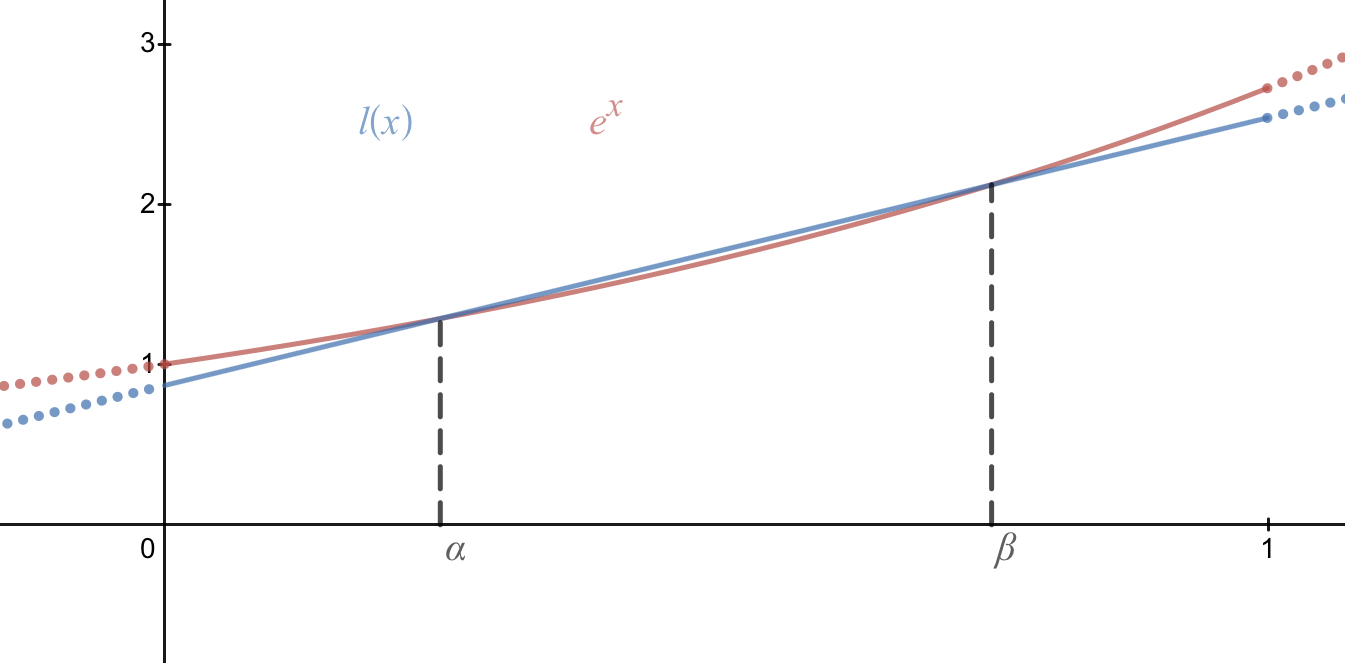
\includegraphics[width=14cm]{hw2_images/desmos12.jpg}\]
We want to minimize the following
\[I = \int_0^1 |e^x - \ell(x)| dx = \int_0^{\alpha} (e^x - \ell(x)) dx + \int_{\alpha}^{\beta} (\ell(x) - e^x) dx + \int_{\beta}^1 (e^x - \ell(x)) dx.\]
If we let $\ell(x) = mx+b$, the following evaluates to
\begin{equation*}
    \begin{split}
        I &= \left[e^x - \frac{m}{2}x^2 - bx\right]\bigg|_0^{\alpha} + \left[\frac{m}{2}x^2 + bx - e^x\right]\bigg|_{\alpha}^{\beta} + \left[e^x - \frac{m}{2}x^2 - bx\right]\bigg|_{\beta}^1 \\
        &= \left(e^{\alpha} - \frac{\alpha^2}{2}m - \alpha b - 1\right) + \left(\frac{\beta^2}{2}m + \beta b - e^{\beta}\right) - \left(\frac{\alpha^2}{2}m + \alpha b - e^{\alpha}\right) \\
        & \qquad \qquad \qquad + \left(e - \frac{1}{2}m - b\right) - \left(e^{\beta} - \frac{\beta^2}{2}m - \beta b\right) \\
        &= e^{\alpha} - \frac{\alpha^2}{2}m - \alpha b - 1 + \frac{\beta^2}{2}m + \beta b - e^{\beta} - \frac{\alpha^2}{2}m - \alpha b + e^{\alpha} \\
        & \qquad \qquad \qquad + e - \frac{1}{2}m - b - e^{\beta} + \frac{\beta^2}{2}m + \beta b
    \end{split}
\end{equation*}
\[F(m,b) = I = \left(\beta^2 - \alpha^2 - \frac{1}{2}\right)m + \left(2\beta - 2\alpha - 1\right)b + \left(2e^{\alpha} - 2e^{\beta} + e - 1\right)\]
\[\frac{\partial F}{\partial m} = \beta^2 - \alpha^2 - \frac{1}{2} = 0 \Longrightarrow (\beta - \alpha)(\beta + \alpha) = \frac{1}{2}\]
\[\frac{\partial F}{\partial b} = 2\beta - 2\alpha - 1 = 0 \Longrightarrow \beta - \alpha = \frac{1}{2}\]
Therefore we have,
\[\alpha = \frac{1}{4} \text{  and  } \beta = \frac{3}{4}.\]
Now
\[m = \frac{e^{\beta} - e^{\alpha}}{\beta - \alpha} = 2\left(e^{3/4} - e^{1/4}\right)\]
which means that
\[y = 2\left(e^{3/4} - e^{1/4}\right)x + b \Longrightarrow e^{1/4} = \frac{1}{2}e^{3/4} - \frac{1}{2}e^{1/4} + b \text{, and}\]
\[b = \frac{1}{2}\left(3e^{1/4} - e^{3/4}\right).\]
Therefore,
\[\ell(x) = 2\left(e^{3/4} - e^{1/4}\right)x + \frac{1}{2}\left(3e^{1/4} - e^{3/4}\right) \quad \text{minimizes (11).}\]

\begin{itemize}
    \item[{\textbf{-13-}}] \textbf{(Another alternative approximation problem.)}  Find a linear function $\ell(x)$ such that
    \begin{equation}
        \max_{0 \leq x \leq 1} |e^x - \ell(x)| = \min.
    \end{equation}
\end{itemize}
We know that our function $\ell(x)$ will intersect $e^x$ twice, say at $\alpha$ and $\beta$.  However, we won't focus on these values all that much.  The idea is that the maximum error will occur at one of these intervals.  We wish to minimize the maximum error, to do this the maximum error on each interval \([0, \alpha], [\alpha, \beta], \text{and} [\beta, 1]\) must be identical.  We can always adjust the line to reduce the error.  We can see what this looks like, qualitatively, below.
\[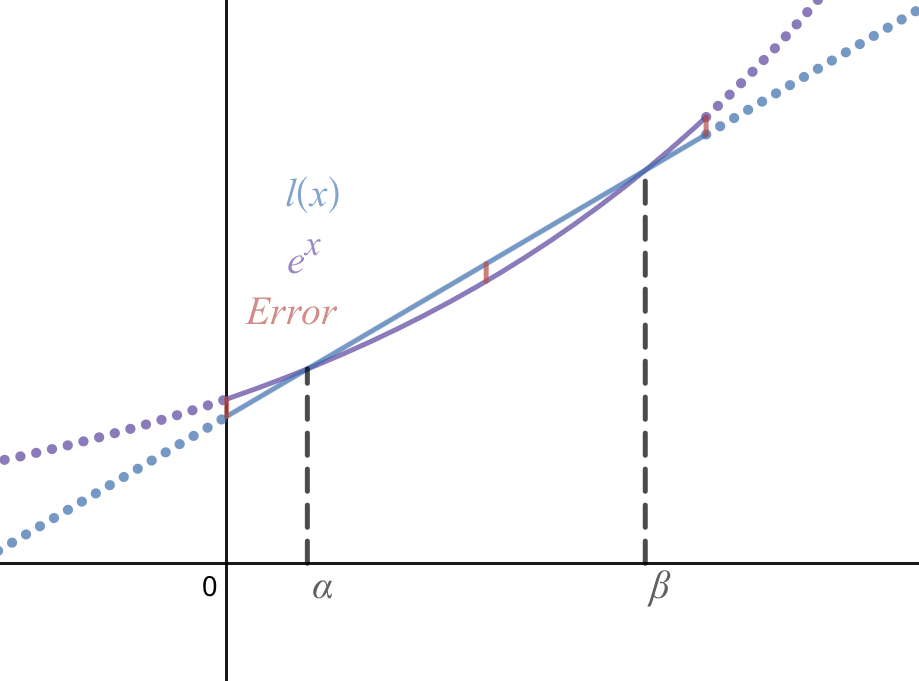
\includegraphics[height=7cm]{hw2_images/desmos13.jpg}\]
We know that based on the shape of $e^x$ on the interval, the minimized maximum error will occur at $x=0, x=1$ and some $\hat{x}$ on the interval $[\alpha, \beta]$.  If we let $\ell(x) = mx+b$ and let $E$ denote the minimized maximum error, then we have the following system,
\[e^0 - (m(0) + b) = E\]
\[e^{\hat{x}} - (m\hat{x} + b) = -E\]
\[e^1 - (m(1) + b) = E\]
We also note that \(E^{\prime}(\hat{x}) = e^{\hat{x}} - m = 0 \Leftrightarrow e^{\hat{x}} = m \Leftrightarrow \hat{x} = \ln (m)\).  Solving the system we have,
\begin{align*}
    e - m - b &= E \\
    (-) \quad 1 - b &= E
\end{align*}
\[\Longrightarrow \quad e - 1 - m = 0 \quad \Longleftrightarrow \quad m = e - 1\]
\begin{align*}
    e - m - b &= E \\
    (+) \quad e^{\hat{x}} - m\hat{x} - b &= -E
\end{align*}
\[\Longrightarrow \quad e + e^{\hat{x}} - m - m\hat{x} - 2b = 0 \]
\begin{equation*}
    \begin{split}
        \Longrightarrow \quad 2b &= e + e^{\hat{x}} - m - m\hat{x} \\
        b &= \frac{1}{2}\left(e - m\hat{x}\right) \\
        &= \frac{1}{2}\left(e - (e - 1)\ln(e - 1)\right) \\
        &= \frac{1}{2}\left(e - e\ln(e - 1) + \ln(e - 1)\right)
    \end{split}
\end{equation*}

Thus, \(\ell(x) = (e - 1)x + \frac{1}{2}\left(e - e\ln(e-1) + \ln(e-1)\right)\) minimizes our function.

\pagebreak

\section{Appendix}

\begin{itemize}
    \item[{\textbf{-A-}}] Python Code for Graphs in problem 1.
\end{itemize}
\begin{lstlisting}[language=Python]
    import matplotlib.pyplot as plt
    import numpy as np
    from math import factorial

    t = np.linspace(-10, 10, 1000)

    # I need this one for the ln function since I don't know how to
    # deal with singularity of -1
    t_ln = np.linspace(-0.9999, 10, 1000)

    # Define e^x
    def f(x):
        return np.exp(x)

    # Define ln(x+1)
    def g(x):
        return np.log(x+1)

    # Define taylor poly for e^x
    def p(x,n):
        if n == 0:
            return 1
        else:
            return ((x**n) / factorial(n)) + p(x, n-1)

    # Define taylor poly for ln(x+1)
    def q(x,n):
        if n == 1:
            return x
        else:
            return (-1)**(n-1) * factorial(n-1)*x**n / factorial(n)
                + q(x, n-1)

    # For subplots
    fig, ax = plt.subplots(2, 4, figsize=(10,5))
    i = 0
    for n in range(1, 23, 3):
        # print(n)
        test = ax[i // 4, i % 4]
        test.plot(t, f(t), color='blue', label='e^x')
        test.plot(t, p(t, n), color='blue', linestyle='--', label='p')
        test.plot(t_ln, g(t_ln), color='red', label='ln(1+x)')
        test.plot(t, q(t, n), color='red', linestyle='--', label='q')
        test.set_ylim(-10, 10)
        test.set_title(f'Degree {n}')
        i+=1

    fig.show()
\end{lstlisting}

\begin{itemize}
    \item[{\textbf{-B-}}] Python Code for Errors in problem 1.
\end{itemize}
\begin{lstlisting}[language=Python]
    import numpy as np
    from math import factorial
    import matplotlib.pyplot as plt

    def f(x):
        return np.exp(x)

    # Define ln(x+1)
    def g(x):
        return np.log(x+1)

    # Define taylor poly for e^x
    def p(x,n):
        if n == 0:
            return 1
        else:
            return ((x**n) / factorial(n)) + p(x, n-1)

    # Define taylor poly for ln(x+1)
    def q(x,n):
        if n == 1:
            return x
        else:
            return (-1)**(n-1) * factorial(n-1)*x**n / factorial(n)
                + q(x, n-1)

    def error_f(x,n):
         return abs(f(x) - p(x, n))

    def error_g(x,n):
        if x <= -1:
            return 'undefined'
        else:
            return abs(g(x) - q(x, n))

    # Parameters for graph
    x = 1
    n = 14

    domain = [i for i in range(1, n+1)]
    codomain_f = [error_f(x, i) for i in range(1, n+1)]
    codomain_g = [error_g(x, i) for i in range(1, n+1)]

    print("e^x errors:")
    print('----------')
    for i in range(0,n):
        print(f'degree {i+1}: {codomain_f[i]}')
    print()

    print("ln errors:")
    print('----------')
    for i in range(0,n):
        print(f'degree {i+1}: {codomain_g[i]}')

    x_list = [1, 1.1, 1.2, 1.3, 1.4, 1.5]
    fig, ax = plt.subplots(2, 3, figsize=(10, 7))

    for j in range(6):
        codomain_f = [error_f(x_list[j], i) for i in range(1, n + 1)]
        codomain_g = [error_g(x_list[j], i) for i in range(1, n + 1)]
        test = ax[j // 3, j % 3]
        x_ticks = np.arange(1, n+1, 1)
        test.set_xticks(x_ticks)
        test.set_title(f'Error at x={x_list[j]}')
        test.scatter(x=domain, y=codomain_f, color='blue',
            label='e^x approximation error')
        test.scatter(x=domain, y=codomain_g, color='red',
            label='ln approximation error')
        test.set_xlabel('degree n')
        test.set_ylabel('error')


    fig.show()
\end{lstlisting}

\begin{itemize}
    \item[{\textbf{-C-}}] Python Code for Runtimes in problem 3.
\end{itemize}
\begin{lstlisting}[language=Python]
    from math import sin
    import time

    # My first program to test how many steps it takes to get epsilon
    # distance from 0
    i = 0
    x = 1
    tolerance = 0.001
    flag1 = time.process_time()
    while True:
        i += 1
        x = sin(x)
        if x < tolerance:
            flag2 = time.process_time()
            break
    time_length = flag2-flag1
    print(f'error: {x}\n', f'steps: {i}\n', f'time: {time_length}')
    print()
    # Code to look at how at effects of rounding errors.
    i = 0
    x = 1
    n = 300
    rounding = 3

    for step in range(n):
        i += 1
        x = round(sin(x), rounding)
        print(f'{step}: {x}')
\end{lstlisting}

\begin{itemize}
    \item[{\textbf{-D-}}] Python Code for Interpolants in problem 9.
\end{itemize}
\begin{lstlisting}[language=Python]
    import matplotlib.pyplot as plt
    import numpy as np
    # from scipy import interpolate, linalg

    # Define a linespace (or domain)
    domain = np.linspace(-5, 5, 1000)

    # Define the function
    def f(x):
        return 1/(1+x**2)

    # Interpolate with different degree polynomials
    for n in range(1,21):
        h = 10 / n

        # creating our nodes
        x = [-5+i*h for i in range(n+1)]
        y = [f(i) for i in x]

       # Creating the Vondermond Matrix
        rows = []
        for i in x:
            row = [i**j for j in range(n+1)]
            rows.append(row)

        # Create my system that needs to be solved
        x_vondermond = np.array(rows)
        y_vondermond = np.array(y)

        # Solve the system of equations!
        sol = np.linalg.solve(x_vondermond, y_vondermond)

        # I built a function recursively.
        def poly(x, n):
            if n == 0:
                return sol[0]
            else:
                return sol[n]*x**n + poly(x, n-1)

        # Find the max error
        error = [abs(f(i)-poly(i, n)) for i in domain]
        max_error = max(error)
        max_error_index = error.index(max_error)
        print(f"Degree {n} Max Error: {max_error}")
        plot_value = -5 + max_error_index/100
        # You divide by 1000 and then multiply by 10--think about it...

        # Plot the results
        plt.plot(domain, f(domain), label='function', color='blue')
        plt.plot(domain, poly(domain,n), label='Interpolant')
        plt.ylim([-0.5, 1.5]) #To fix plotting frame.
        plt.text(-2, 1.25, f'Max Error: {max_error}')
        plt.vlines(x=plot_value, ymin=min(f(plot_value),
            poly(plot_value, n)), ymax=max(f(plot_value),
            poly(plot_value, n)), linestyle='--', color='red',
            label="Max Error")
        plt.title(f"Degree {n} Interpolation")
        plt.legend(loc=8)
        # plt.savefig(f'degree_{n}.jpg', bbox_inches='tight')
        plt.show()
\end{lstlisting}

\begin{itemize}
    \item[{\textbf{-E-}}] Python Code for Interpolants in problem 10.
\end{itemize}
\begin{lstlisting}[language=Python]
    # Chebycheff Polynomial
    import matplotlib.pyplot as plt
    import numpy as np
    # from scipy import interpolate, linalg

    # Define a linespace (or domain)
    domain = np.linspace(-5, 5, 1000)

    # Define the function
    def f(x):
        return 1/(1+x**2)

    # Interpolate with different degree polynomials
    for n in range(1, 21):

        # creating our nodes
        x = [5*np.cos(i*np.pi/n) for i in range(n+1)]
        y = [f(i) for i in x]

        # Creating the Vondermond Matrix
        rows = []
        for i in x:
            row = [i**j for j in range(n+1)]
            rows.append(row)

        # Create my system that needs to be solved
        x_vondermond = np.array(rows)
        y_vondermond = np.array(y)

        # Solve the system of equations!
        sol = np.linalg.solve(x_vondermond, y_vondermond)

        # I built the function recursively.
        def poly(x, n):
            if n == 0:
                return sol[0]
            else:
                return sol[n]*x**n + poly(x, n-1)

        # Find the max error
        error = [abs(f(i)-poly(i, n)) for i in domain]
        max_error = max(error)
        max_error_index = error.index(max_error)
        print(f"Degree {n} Max Error: {max_error}")
        plot_value = -5 + max_error_index/100
        # You divide by 1000 and then multiply by 10--think about it...

        # Plot the results
        plt.plot(domain, f(domain), label='function', color='blue')
        plt.plot(domain, poly(domain,n),
            label='Chebycheff Interpolant')
        plt.text(0, 0.1, f'Max Error: {max_error}',
            horizontalalignment='center', verticalalignment='center')
        plt.vlines(x=plot_value, ymin=min(f(plot_value),
            poly(plot_value, n)), ymax=max(f(plot_value),
            poly(plot_value, n)), linestyle='--', color='red',
            label="Max Error")
        plt.title(f"Degree {n} Chebycheff Interpolation")
        plt.legend(loc=1)
        # plt.savefig(f'chebycheff_{n}.jpg', bbox_inches='tight')
        plt.show()
\end{lstlisting}



\end{document}
